\title{Craterbase: Proposing an open lunar feature navigation pipeline and database}
\author{
        J.~O.~``Juno''~Woods,~Ph.D. \\
        Director of Engineering Research \& Strategy\\
        Open Lunar Foundation\\
        San Francisco, California
}
\date{\today}
%\date{November~19,~2019}

\documentclass[12pt]{article}
\usepackage{natbib}
\usepackage{amsmath}
\usepackage{hyperref}
\bibliographystyle{unsrtnat}
\usepackage{graphicx}

\begin{document}
\maketitle

\section{Introduction}
With an average of 384,400 kilometers between the Earth and the Moon, radiometric measurements of a spacecraft's range and range-rate are a both an expensive and currently essential commodity, both technically and monetarily. Without a counterpart spacecraft functioning as a relay, these measurements are wholly unavailable for transits behind the Moon. Moreover, these services are capacity-limited, as a ground station must be pointed at the spacecraft it aims to measure, and preclude full autonomy, because measurements are taken on the ground. While both the European Space Agency and the National Aeronautics and Space Administration have expressed interest in a lunar analogue of the various Earth global navigation satellite systems (\textsc{gnss}), a variety of optical navigation (\textsc{opnav}) strategies may be leveraged for fully autonomous navigation in the vicinity of the Moon \citep{Christian2009}. Many of these same optical strategies have also proved useful for missions to other bodies, such as Mars and asteroids.

During transit, measurements can be made between a known star and the horizon or a landmark of the Moon (or Earth) within a few kilometers, a strategy demonstrated aboard Apollo~8 \citep{Christian2009,Hoag1976}, though there are a few challenges surrounding the comparative brightness of the planet and star. Horizon-based optical navigation provides increasingly precise measurements as the planet grows larger in the camera field of view \citep{Christian2016,Christian2017}. A variety of strategies may be utilized once terrain features are visible, such as visual odometry, delta-position, and terrain-relative navigation --- the last of which is the focus of this manuscript. Finally, hazard-relative strategies may be adopted for the final approach. All of these techniques are achievable using a camera, a simple, low-cost, low-power technology.

%While other technologies, such as radars, lidars, and laser altimeters may also provide measurements during descent and landing, there are few other good options for the lunar orbit segment of the trajectory aside from %measurements of stellar occultation by the planet \citep{Keenan1962,Landgraf2006,Psiaki2007,Christian2009} and 
%terrain-relative navigation (\textsc{trn}). % The former provides on the order of a kilometer of error, but can be utilized \citep{Landgraf2006}, and the latter

The most typical instantiation of terrain-relative navigation, or \textsc{trn}, involves measuring the bearing of surface features of known positions, and provides the spacecraft with a few tens or hundreds of meters of position error \citep{Christensen2011}. Terrain features exist at all scales, though the feature catalogue must ultimately be dependent upon the sensor resolution of orbital assets such as the Lunar Reconnaissance Orbiter Camera (about 50 cm per pixel), or landers that have imaged at lower altitudes. A feature catalogue is also limited by registration accuracy or map tie error, since each feature's position must be estimated with respect to a lunar-fixed frame (which itself includes some error) during catalogue construction.

Craters are a commonly catalogued feature, as reviewed by \citet{Robbins2019}, whose own database includes around two million such features. Such indices are primarily oriented toward planetary geology and other science purposes rather than navigation. Prior to the 2009 launch of the Lunar Reconnaissance Orbiter, they were largely constructed on the basis of imagery, and \citet{Salamuniccar2008} noted substantial map tie errors in similarly constructed Martian crater maps. Starting in 2010, the existence of digital terrain models and ready access to far-side imagery generated a rapid increase in catalogue sizes --- but also meant that many craters were identified using non-visual cues. It is also unusual for these databases to include craters smaller than 1 kilometer in diameter. Crater age correlates with crater size, and older craters are visually `noisier.' As such, these newer databases are not optimally configured for optical navigation.

Craters are the preferred feature type for most spacecraft terrain-relative navigation needs, due largely to their geometric nature (at least compared to other feature types) and fairly uniform distribution across the lunar surface.

Owing to the different motivations and criteria used by crater detection algorithms, or \textsc{cda}s, there exists no single survey of strategies, and little consensus on the best approaches. \citet{Christian2020} summarize navigation-relevant research, noting that the goals often differ between scientific and navigation algorithms. Scientific \textsc{cda}s are expected to produce exhaustive lists, whereas for navigation, sensitivity is unimportant, and the goals are speed and sufficient robustness that human supervision is unnecessary. Moreover, many \textsc{cda}s incorrectly assume craters are circular. While \citet{Salamuniccar2008} propose a framework for comparing the results of different \textsc{cda}s, their metric offers little assistance with lighting and perspective differences. Indeed, a recent comparison used a separate set of quantitative metrics but evaluated lighting and perspective robustness only qualitatively \citep{Woicke2018}. It is thus not straightforward to identify an appropriate \textsc{cda} for our purposes.

Whereas detection aims to locate craters in images, the goal of matching is to link such craters to their entries in catalogues. \citet{Christian2020} both reviews crater matching algorithms and identifies an efficient, mathematically rigorous strategy for matching based on invariant theory.

With the crater matching aspect largely sewn up, we turn back to crater detection and databases. We know of only one database for crater-based \textsc{trn}. \textsc{Dlr} researchers have constructed an end-to-end crater navigation system, CNav, which demonstrates crater detection and matching, and includes a non-public crater navigation database \citep{Maass2016,Maass2020}. Likewise, Intuitive Machines, a Commercial Lunar Payload Services provider, is working on an open source optical navigation system called Thin\textsc{vpu} \citep{Stewart2020}.

Of greater interest to us than a navigation database, however, is the pipeline for producing such a catalogue (Fig~\ref{fig:flowchart}). We expect that the algorithm employed for feature detection in navigation flight software would need to share a great deal of similarity with the algorithm used for database construction, a common design pattern for feature matching. Because robust feature detection for this purpose is not a solved problem, the production of a navigation feature database alone is insufficient and would suffer from near-term obsolescence. Efforts toward such a pipeline could result in a number of databases, each generated with different extraction algorithms or settings.

\subsection{A pipeline and database as a public utility}
A \textsc{gnss} constellation such as \textsc{gps} is at its core a public utility (and hence a public good). For the most part, \textsc{gps} cannot selectively exclude certain users (short of being shut off entirely). Because the \textsc{gps} signal is a broadcast, the system is also non-subtractable (or non-rival); its use by some does not diminish the utility to others.

A pipeline for generating feature databases is likewise a public utility, as are the resulting databases. Their nature as data implies that they are non-excludable and non-subtractable.

Worth considering is the licensing of such a system. Open source licenses are often classified on a spectrum from restrictive to permissive. The more restrictive \textsc{gnu} General Public License (\textsc{gpl}) 3.0 requires that source code be distributed along with binaries. With more permissive licenses, such as \textsc{mit} or \textsc{bsd}, derivative source code need not be released. The use-case for the software often dictates the license. For example, a commonly used library like Open\textsc{cv} might be released under a permissive license (in this case the \textsc{bsd} 3-clause license) so it can be easily incorporated into commercial products that only use the library incidentally. On the other hand, the Linux kernel is released under a more restrictive license (\textsc{gpl} v2) to ensure that derivative products remain public.

We believe that the proposed pipeline ought to be released under a custom restrictive license with three goals:
\begin{enumerate}
\item Source code for modified pipelines must also be released under a restrictive license.
\item Resulting databases must be made available to the public.
\item The source code for feature extraction algorithms used with the pipeline must be made available to the public.
\end{enumerate}
With appropriate licensing, we can incentivize contribution to a pipeline that may one day provide navigation databases for use on planets other than the Moon, with features that are more efficient to extract than ellipses.


\begin{figure}
\center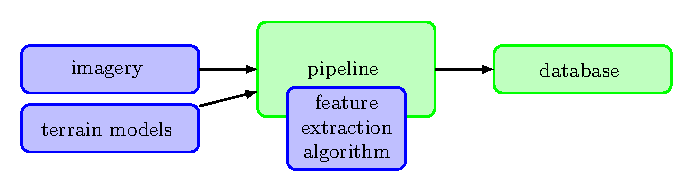
\includegraphics{flowchart.pdf}
\caption{\label{fig:flowchart}\textbf{Our proposed pipeline generates feature databases using a provided feature detection algorithm, planetary imagery, and optional terrain models.} The pipeline itself ought to be licensed under a viral license that also governs the release of the database, regardless of the licensing of the components in blue (imagery, terrain models, and feature algorithm).}
\end{figure}


\bibliography{craterbase}
\end{document}